\documentclass{sigplanconf}
\usepackage{amssymb}
\usepackage{graphicx}
\usepackage{amsmath}
\usepackage{mathptmx}
\usepackage{stmaryrd}
\usepackage{hyperref}
\usepackage{alltt}
\usepackage{url}
\usepackage{float}
\usepackage{style/utils}
\usepackage{style/code}
\usepackage{style/proof}
\usepackage{style/judgements}

% -----------------------------------------------------------------------------
\begin{document}

\exclusivelicense
\conferenceinfo{FHPC~'14}{September 4, 2014, Gothenburg, Sweden}
\copyrightyear{2014}
\copyrightdata{978-1-4503-3040-4/14/09}
\doi{2636228.2636235}
 \pagenumbering{gobble} 

% ACM 978-1-4503-3040-4/14/09 $15.00.
% http://dx.doi.org/10.1145/2636228.2636235 

\title{Fusing Filters with Integer Linear Programming}

\authorinfo{ 
  Amos Robinson$^\dagger$ 
  \and Ben Lippmeier$^\dagger$
  \and Gabriele Keller$^\dagger$ 
}{
  \vspace{5pt}
  \shortstack{
    $^\dagger$Computer Science and Engineering \\
    University of New South Wales, Australia \\[2pt]
    \textsf{\{amosr,benl,keller\}@cse.unsw.edu.au}
  }
}

\maketitle
\makeatactive

\begin{abstract}
The key to compiling functional, collection oriented array programs into efficient code is to minimise memory traffic.
Simply fusing subsequent array operations into a single computation is not sufficient; we also need to cluster \emph{separate} traversals of the same array into a single traversal.
Previous work demonstrated how Integer Linear Programming (ILP) can be used to cluster the operators in a general data-flow graph into subgraphs, which can be individually fused.
However, these approaches can only handle operations which preserve the size of the array, thereby missing out on some optimisation opportunities.
This paper addresses this shortcoming by extending the ILP approach with support for size-changing operations, using an external ILP solver to find good clusterings.
\end{abstract}


\category
	{D.3.4}
	{Programming Languages}
	{Processors---Compilers; Optimization}

\terms
	Languages, Performance

\keywords
	Arrays; Fusion; Haskell

%!TEX root = ../Main.tex
\section{Introdution}

The Haskell library ecosystem is blessed with a multitude of libraries for writing streaming data flow programs. Stand out examples include iteratee CITE, enumerator CITE, conduit CITE and pipes CITE. These libraries are based around ... and more recent examples such as pipes provide a useful set of algebraic equivalences that give a clean mathematical structure to the provided mathemetical structure.

Libraries such as iteratee and enumerator are typically used to deal with data sets that do not fit in main memory, as the constant space guarantee ensures that the program will run to completion without suffering an out-of-memory error. However, current computing platforms use multi-core processors, the programming models provided by such streaming libraries do not also provide a notion of \emph{parallelism} to help deal with the implied amount of data. They also lack support for branching data flows where produced streams can be consumed by several consumers without the programmer needing to had fuse them.

We provide several techniques that increase the scope of programs that can be written in such libraries. Our target applications concern \emph{medium data}, meaning data that is large enough that it does not fit in the main memory of a normal desktop machine, but not so large that we require a cluster of multiple physical machines. For a lesser amount of data one could simply load the data into main memory and use an in-memory array library such as CITE or CITE. For greater data one needs to turn to a distributed system such as Hadoop or Spark and deal with the unreliable network and lack of shared memory. Repa Flow targets the sweet middle ground.

We make the following contributions:

\begin{itemize}
\item Our parallel data flows consist of a bundle of streams, where each stream can process a separate partition of a data set on a separate processor core.

\item Our API uses polarised flow endpoints (@Sources@ and @Sinks@) to ensure that programs run in constant space. We demonstrate how this standard technique can be extended to branching data flows, where produced flows are consumed by multiple consumers.

\item The data processed by our streams is chunked so that each operation processes several elements at a time. We show how to design the core API in a generic fashion so that chunk-at-a-time operators can interoperate smoothly with element-at-a-time operators.
\TODO{We don't support leftovers}

\item We show how to use Continuation Passing Style to provoke the Glasgow Haskell Compiler into applying stream fusion across chunks processed by independent flow operators. For example, the map-map fusion on flows arises naturally from map-map fusion rule on chunks (arrays) of elements.
\end{itemize}

Our work is embodied in Repa Flow, which is available on Hackage. \TODO{Specify the relationship to previous work on Repa}. This is a new layer on the original delayed arrays of our original Repa library.


%!TEX root = ../Main.tex

\begin{figure*}[ht!]
\begin{center}
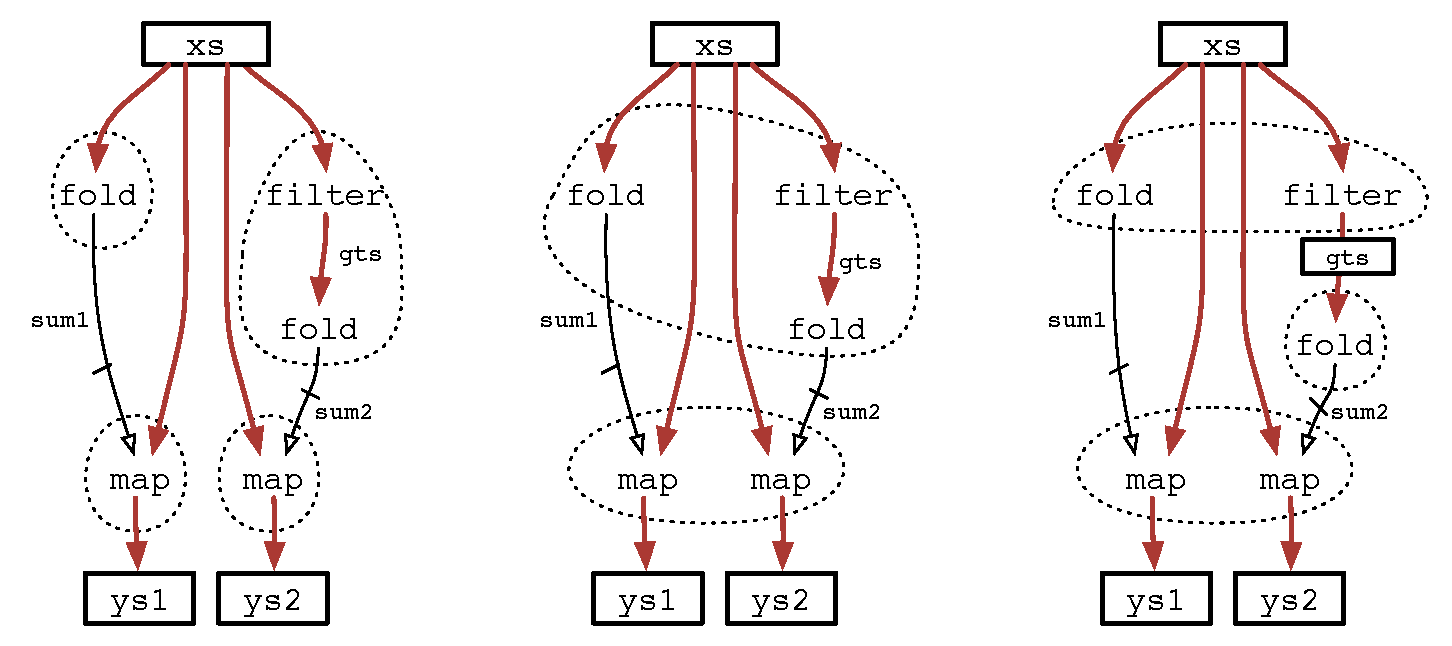
\includegraphics[scale=0.5]{figures/ex1-compare.pdf}
\end{center}
\caption{Clusterings for normalize2 example: with stream fusion; our system; best imperative system}
\label{f:normalize2-clusterings}
\end{figure*}


% -----------------------------------------------------------------------------
\section{Combinator Normal Form}
\label{s:CombinatorNormalForm}
Input programs are expressed in \emph{Combinator Normal Form} (CNF), which is a textual description of the data flow graph. The grammar for CNF is given in Figure~\ref{f:CombinatorNormalForm}. The @normalize2@  example on the previous page is in CNF,  as is the matching data flow graph for @normalize2@ in Figure~\ref{f:normalize2-clusterings}. Our data flow graphs are similar to Loop Communication Graphs (LCGs) from related work in imperative array fusion~\cite{gao1993collective}. We name edges after the corresponding variable from the CNF form, and edges which are fusion preventing are drawn with a dash through them (as per the edge labeled @sum1@ in Figure~\ref{f:normalize2-clusterings}). In data flow graphs, we tend to elide the worker functions to combinators when they are not important to the discussion --- so we don't show the @(+)@ operator on each use of @fold@.

Clusters of operators that are fused into single imperative loops are indicated by dotted lines, and we highlight materialized arrays by drawing them in boxes. In Figure~\ref{f:normalize2-clusterings}, the variables @xs@, @ys1@ and @ys2@ are always in boxes, as these are the material input and output arrays of the program. However, in the graph on the far right hand side, @gts@ has also been materialized because in this version, the producing and consuming operators (@filter@ and @fold@) have not been fused. In Figure~\ref{f:CombinatorNormalForm}, note that the bindings have been split into those that produce scalar values ($sbind$), and those that produce array values ($abind$). These groupings are represented as open and closed arrow-heads in Figure~\ref{f:normalize2-clusterings}.

Most of our array combinators are standard, and suggestive types are given at the bottom of Figure~\ref{f:CombinatorNormalForm}. The $@map@_n$ combinator takes a worker function, $n$ arrays of the same length, and applies the worker function to all elements at the same index. As such, it is similar to Haskell's @zipWith@, with an added length restriction on the argument arrays. The @generate@ combinator takes an array length and a worker function, and creates a new array by applying the worker to each index. The @gather@ combinator takes an array of elements, an array of indices, and produces the array of elements that are positioned at each index. In Haskell, this would be @gather arr ixs = map (index arr) ixs@. The @cross@ combinator returns the cartesian product of two arrays. 

The exact form of the worker functions is left unspecified, as it is not important for the discussion. We assume workers are pure, can at least compute arithmetic functions of their scalar arguments, and index into arrays in the environment. We also assume that each CNF program considered for fusion is embedded in a larger host program which handles file IO and the like. Workers are additionally restricted so they can only directly reference the \emph{scalar} variables bound by the local CNF program, though they may reference array variables bound by the host program. All access to locally bound array variables is via the formal parameters of array combinators, which ensures that all data dependencies we need to consider for fusion are explicit in the data flow graph.

The @external@ binding invokes a host library function that can produce and consume arrays, but not be fused with other combinators. All arrays passed to and returned from host functions are fully materialised. External bindings are explicit \emph{fusion barriers}, which force arrays and scalars to be fully computed before continuing. 

Finally, note that @filter@ is only one representative size changing operator. We can handle more complex functions such as @unfold@ in our framework, but we stick with simple filtering to aid the discussion.


%!TEX root = ../Main.tex
\begin{figure}
\begin{tabbing}
MMMM        \= MM \= MMMMMMMMM \= \kill
$\scalar$    \> $\to$ \> (scalar variable) \\
$\arrayz$     \> $\to$ \> (array variable)  \\
$f$         \> $\to$ \> (worker function) \\
$\fun$       \> $\to$ \> $f~\scalar\ldots$
\\[2ex]
$\bind$      \> @::=@ \> $\scalar$ \> $=~\sbind$ \\
            \> $~|$  \> $\arrayz$  \> $=~\abind$ \\
            \> $~|$  \> $\scalar\ldots,\arrayz\ldots$ \> $=~@external@~\scalar\ldots~\arrayz\ldots$
\end{tabbing}

\begin{tabbing}
MMMM        \= MM \= MMMMM \= MMMMMM \= M \= MMMM \= MMMMMM \= \kill
$\sbind$     \> @::=@ \> $@fold@$     \> $\fun~~ \arrayz$
\\[1ex]

$\abind$     \> @::=@ \> $@map@_n$    \> $\fun~~ \arrayz^n$ 
            \> $~|$  \> $@filter@$   \> $\fun~~ \arrayz$   \\
            \> $~|$  \> $@generate@$ \> $\scalar~~ \fun$  
            \> $~|$  \> $@gather@$   \> $\arrayz~~ \arrayz$ \\
            \> $~|$  \> $@cross@$    \> $\arrayz~~ \arrayz$
\\[1ex]
$\program$  \> @::=@ \> $f~\scalar\ldots~\arrayz\ldots~=$ \\
            \>          \> $@let@~\bind\ldots$                  \\
            \>          \> $@in@~(\scalar\ldots,~\arrayz\ldots)$
\\[3ex]
$@fold@$     \> $:~ (a \to a \to a) \to @Array@~~ a \to a$     \\
$@map@_n$    \> $:~ (\{a_i          \to\}^{\;i\; \gets 1 \dots n}~~ b)  \to
                       \{@Array@~~ a_i \to\}^{\;i\; \gets 1 \dots n}~~ @Array@~~ b$ \\
$@filter@$   \> $:~ (a \to @Bool@) \to @Array@~~ a \to @Array@~~ a$      \\
$@generate@$ \> ~~ $:~ @Nat@ \to (@Nat@ \to a) \to @Array@~~ a$          \\
$@gather@$   \> ~~ $:~ @Array@~~ a \to @Array@~~ @Nat@  \to @Array@~~ a$ \\
$@cross@$    \> ~~ $:~ @Array@~~ a \to @Array@~~ b ~~~~ \to @Array@~~ (a, b)$
\end{tabbing}
\caption{Combinator normal form}
\label{f:CombinatorNormalForm}
\end{figure}




%!TEX root = ../Main.tex
\section{Size Inference}
Before performing fusion proper, we must infer the relative sizes of each array in the program. We achieve this with a simple constraint based inference algorithm, which we discuss in this section. Size inference has been previously described in the context of array fusion by Chatterjee~\cite{chatterjee1991size}. In constrast to our algorithm, \cite{chatterjee1991size} does not support size changing functions such as filter.
If size inference fails, the programs may still be compiled, but fusion is not performed.

Although our constraint based formulation of size inference is reminiscent of type inference for HM(X)~\cite{odersky1999type}, there are important differences. Firstly, our type schemes include existential quantifiers, which express the fact that the sizes of arrays produced by filter operations are unknown in general. This is also the case for @generate@, where the result size is data dependent. HM(X) style type inferences use the $\exists$ quantifier to bind local type variables in constraints, and existential quantifiers do not appear in type schemes. Secondly, our types are first order only, as program graphs cannot take other program graphs as arguments. Provided we generate the constraints in the correct form, solving them is straightforward.


% -----------------------------------------------------------------------------
\begin{figure}
\begin{tabbing}
MMMMMMMM \= MM  \= MM \= MMMMMM \= \kill
\textbf{Size Type}
\> $\tau$   \> @::=@  \> $k$                  \> (size variable)       \\
\>          \> $~|$   \> $\tau \times \tau$   \> (cross product)
\end{tabbing}

\begin{tabbing}
MMMMMMMM \= MM  \= MM \= MMMMMM \= \kill
\textbf{Size Constraint}
\> $C$      \> @::=@  \> $\true$               \> (trivially true)      \\
\>          \> $~|$   \> $k = \tau$           \> (equality constraint) \\
\>          \> $~|$   \> $C \wedge C$         \> (conjunction)
\end{tabbing}

\begin{tabbing}
MMMMMMMM \= MM  \= MM \= MMMMMM \= \kill
\textbf{Size Scheme}
\> $\sigma$ \> @::=@  
        \> $\forall \ov{k}.~ \exists \ov{k}.~ (\ov{ x : \tau }) \to (\ov{x : \tau})$
\end{tabbing}

\caption{Sizes, Constraints and Schemes}
\label{f:constraints}
\end{figure}


\newcommand{\constr}[1]{\llbracket #1 \rrbracket}


% -----------------------------------------------------------------------------
\subsection{Size Types, Constraints and Schemes}
\label{s:SizeTypes}
Figure~\ref{f:constraints} shows the grammar for size types, constraints and schemes. A size scheme is like a type constraint from Hindley-Milner type systems, except that it only mentions the size of each input array, instead of the element types as well.

A size may either be a variable $k$ or a cross product of two sizes. We use the latter to represent the result size of the @cross@ operator discussed in the previous section. Constraints may either be trivially $\true$, an equality $k = \tau$, or a conjunction of two constraints $C \wedge C$. We refer to the trivially true and equality constraints as \emph{atomic constraints}. Size schemes relate the sizes of each input and output array. For example, the size scheme for the @normalize2@ example from Figure~\ref{f:normalize2-clusterings} is as follows:
$$@normalize2@ ~:_s \forall k. (xs : k) \to (ys_1 : k,~ ys_2 : k)
$$

We write $:_s$ to distinguish size schemes from type schemes.

The existential quantifier appears in size schemes when the array produced by a filter or similar operator appears in the result. For example:
\begin{alltt}
 filterLeft \(:\sb{s}\,\forall\,k\sb{1}.\,\exists\,k\sb{2}.\,(xs\,:\,k\sb{1})\;\to\;(ys\sb{1}\,:\,k\sb{1},\,ys\sb{2}\,:\,k\sb{2})\)
 filterLeft xs
   = let ys1 = map (+ 1)   xs
         ys2 = filter even xs
     in (ys1, ys2)
\end{alltt}

The size scheme of @filterLeft@ shows that it works for input arrays of all sizes. The first result array has the same size as the input, and the second has some unrelated size.

Finally, note that size schemes form but one aspect of the type information that would be expressible in a full dependently typed language. For example, in Coq or Agda we could write something like:
\begin{alltt}
 filterLeft : \(\forall\,k\sb{1}:\,\)Nat\(.\,\exists\,k\sb{2}:\,\)Nat\(.\) 
   Array \(k\sb{1}\) Float \(\to\) (Array \(k\sb{1}\) Float, Array \(k\sb{2}\) Float)
\end{alltt}

However, the type inference systems for fully higher order dependently typed languages typically require quantified types to be provided by the user, and do not perform the type generalization process. In our situation, we need automatic type generalization, but for a first order language only.


% -----------------------------------------------------------------------------
\subsection{Constraint Generation}
The rules for constraint generation are shown in Figure~\ref{f:ConstraintGeneration}. The top level judgment ~~$\SizeF{\program}{\sigma}$~~ assigns a size scheme to a program. It does this by extracting size constraints and then solving them. This rule, along with the constraint solving process is discussed in the next section. The judgment ~~$\SizeB{\Gamma_1}{zs}{b}{\Gamma_2}{C}$ reads: ``Under environment~$\Gamma_1$, array variable $zs$ binds the result of $b$, producing a result environment $\Gamma_2$ and size constraints $C$''. The remaining judgment that extracts constraints from a list of bindings is similar. The environment $\Gamma$ has the following grammar:
$$
\Gamma~ @::=@ ~~\cdot ~~|~~ \Gamma,~ \Gamma ~~|~~ zs : k ~~|~~ k ~~|~~ \exists k
$$

As usual, $\cdot$ represents the empty environment and  $\Gamma,~ \Gamma$
environment concatenation. The element $zs : k$ records the size $k$ of some
array variable $zs$. A plain $k$ indicates that $k$ can be unified with other
size types when solving constraints, whereas $\exists k$ indicates a  \emph{rigid} size variable that cannot be unified with other sizes. We use the $\exists k$ syntax because this variable will also be existentially quantified if it appears in the size scheme of the overall program.

Note that the constraints are generated in a specific form, to facilitate the constraint solving process. For each array variable in the program, we generate a new size variable, like size $k_{zs}$ for array variable $zs$. These new size variables always appear on the \emph{left} of atomic equality constraints. For each array binding we may also introduce unification or rigid variables, and these appear on the \emph{right} of atomic equality constraints.

For example, the final environment and constraints generated for the @normalize2@ example from Section~\ref{s:Introduction} are as follows:
$$
\begin{array}{ll}
       & x : k_{xs},~ gts : k_{gts},~ \exists k_1,~ k_2,~ k_3 
\\
\vdash & \true 
        ~\wedge~  k_{gts} = k_1
        ~\wedge~  \true
\\     &~~~~~~~~ 
          \wedge~  k_{xs}  ~= k_2
        ~ \wedge~  k_{ys1}  = k_2 
        ~ \wedge~  k_{xs}   = k_3
        ~ \wedge~  k_{ys2}  = k_3
\end{array}
$$

Rule~(SProgram) also characterises the programs we accept: a program is \emph{valid} if and only if $\exists \sigma.\ \SizeF{\program}{\sigma}$. 

% -------------------------------------------------------------------
\subsection{Constraint Solving and Generalization}
The top-level rule in Figure~\ref{f:ConstraintGeneration} assigns a size scheme to a program by first extracting size constraints, before solving them and generalizing the result. In the rule, the solving process is indicated by $\textrm{SOLVE}$, and takes an environment and a constraint set, and produces a solved environment and constraint set. As the constraint solving process is both standard and straightforward, we only describe it informally.

Recall from the previous section that in our generated constraints all the size variables named after program variables are on the left of atomic equality constraints, while all the unification and existential variables are on the right. To solve the constraints, we keep finding pairs of atomic equality constraints where the same variable appears on the left, unify the right of both of these constraints, and apply the resulting substitution to both the environment and original constraints. When there are no more pairs of constraints with the same variable on the left, the constraints are in solved form and we are finished.

During constraint solving, all unification variables occuring in the environment can have other sizes substituted for them. In contrast, the rigid variables marked by the $\exists$ symbol cannot. For example, consider the constraints for @normalize2@ mentioned before:
$$
\begin{array}{ll}
       & x : k_{xs},~ gts : k_{gts},~ \exists k_1,~ k_2,~ k_3 
\\
\vdash & \true 
        ~\wedge~  k_{gts} = k_1
        ~\wedge~  \true
\\     &~~~~~~~~ 
          \wedge~  k_{xs}  ~= k_2
        ~ \wedge~  k_{ys1}  = k_2 
        ~ \wedge~  k_{xs}   = k_3
        ~ \wedge~  k_{ys2}  = k_3
\end{array}
$$

Note that $k_{xs}$ is mentioned twice on the right of an atomic equality constraint, so we can substitute $k_2$ for $k_3$. Eliminating the duplicates, as well as the trivially $\true$ terms then yields:
$$
\begin{array}{ll}
       & x : k_{xs},~ gts : k_{gts},~ \exists k_1,~ k_2 
\\
\vdash & k_{gts} = k_1
        ~\wedge~  k_{xs}  ~= k_2
        ~\wedge~  k_{ys1}  = k_2 
        ~\wedge~  k_{ys2}  = k_2
\end{array}
$$

To produce the final size scheme, we look up the sizes of the input and output variables of the original program from the solved constraints and generalize appropriately. This process is determined by the top-level rule in Figure~\ref{f:ConstraintGeneration}. In this case, no rigid size variables appear in the result, so we can universally quantify all size variables.
$$@normalize2@ ~:_s \forall k. (xs : k) \to (ys_1 : k,~ ys_2 : k)
$$

%!TEX root = ../Main.tex

\begin{figure*}
$$
\fbox{$
 \SizeF {\program}{\sigma}
$}
$$
$$
\ruleI  { \begin{array}{ll}
          \SizeL{\{k_i,~ xs_i : k_i \}^{ i \gets 1 .. n }}
                {@let@~ bs~ @in@~ \{ ys_j \}^{j \gets 1 .. m}}
                {\Gamma[ys_j : k'_j]^{j \gets 1.. m}}
                {C}
%
\\        (\Gamma',~ C') = \textrm{SOLVE}(\Gamma,~ C)
\quad     \{ k_i  = s_i \}^{i \gets 1 .. n} \in C'
\quad     \{ k_j' = t_j \}^{j \gets 1 .. m} \in C'
%
\\        \ov{k_a} = \{ k ~|~ k         \in \Gamma' \}  
                        ~\cap~ (\bigcup_{i \gets 1 .. n}\textrm{fv}(s_i))
\quad     \ov{k_e} = \{ k ~|~ \exists k \in \Gamma' \}
                        ~\cap~ (\bigcup_{j \gets 1 .. m}\textrm{fv}(t_j))
\quad     \{ \exists k \notin \Gamma 
                ~|~     \bigcup_{i \gets 1 .. n}\textrm{fv}(s_i)
          \}
          \end{array}
        }
        { \SizeF{f~ \{xs\}^{i \gets 1..n}
                        = @let@~ bs~ @in@~ \{ys\}^{j \gets 1..m}
                }
                { \forall \overline{k_a}.~ 
                  \exists \overline{k_e}.~
                        (\{ xs_i : s_i \}^{i \gets 1..n}) \to
                        (\{ ys_j : t_j \}^{j \gets 1..m})
                }
        }
\quad
\textrm{(SProgram)}
$$

% -------------------------------------------------------------------
$$
\fbox{$
 \SizeL {\Gamma}
        {lets}
        {\Gamma}
        {C}
$}
$$
%
$$
\begin{array}{c}
        \SizeL  {\Gamma}
                {@let@ ~\cdot~ @in@~ exp}
                {\Gamma}
                {\true}
\quad
\textrm{(SNil)}
\hspace{2em}
\ruleI  {\SizeB {\Gamma_1}
                {zs}
                {b}
                {\Gamma_2}
                {C_1}
         \quad
         \SizeL {\Gamma_2}
                {@let@~ bs~ @in@~ exp}
                {\Gamma_3}
                {C_2}
        }
        {\SizeL {\Gamma_1}
                {@let@~ zs~ = b~ ;~ bs~ @in@~ exp}
                {\Gamma_3}
                {C_1 \wedge C_2}
        }
\quad
\textrm{(SCons)}
\end{array}
$$

% -------------------------------------------------------------------
$$
\fbox{$ 
 \SizeB {\Gamma}
        {z}
        {bind}
        {\Gamma}
        {C}
$}
$$
%
$$
\begin{array}{lllll}
% map_n
\SizeB  {\Gamma[xs_i : k_i]^{i \gets 1..n}       &}
        {zs}
        {@map@_n~ f~ \{xs_i\}^{i \gets 1..n}     &}
        {\Gamma,~ zs : k_{zs},~ k'               &}
        {\bigwedge_{i \gets 1..n}
                \{k_i = k'\}
         ~\wedge~ k_{zs} = k'}
\\[1ex]

% filter
\SizeB  {\Gamma                                 &}
        {zs}
        {@filter@~ f~ xs                        &}
        {\Gamma,~ zs : k_{zs},~ \exists k'      &}
        {k_{zs} = k'}
\\[1ex]

% fold
\SizeB  {\Gamma                                 &}
        {x~}
        {@fold@~ f~ xs                          &}
        {\Gamma                                 &}
        {\true}
\\[1ex]

% generate
\SizeB  {\Gamma                                 &}
        {zs}
        {@generate@~ s~ f                       &}
        {\Gamma,~ zs : k_{zs},~ \exists k'      &}
        {k_{zs} = k'}
        \\[1ex]

% gather
\SizeB  {\Gamma[is : k_{is}]                    &}
        {zs}
        {@gather@~ xs~ is                       &}
        {\Gamma,~ zs : k_{zs},~ k'              &}
        {k_{zs} = k',~ k_{is} = k'}
\\[1ex]

% cross
\SizeB  {\Gamma[xs : k_{xs},~ ys : k_{ys}]      &}
        {zs}
        {@cross@~ xs~ ys                        &}
        {\Gamma,~ zs : k_{zs},~ k',~ k''        &}
        {k_{zs} = k' \times k'' 
                ~\wedge~ k_{xs} = k' 
                ~\wedge~ k_{ys} = k''}
\\[1ex]

% external
\SizeB  {\Gamma                                 &}
        {zs}
        {@external@~ \{xs\}^{i \gets 1..n}      &}
        {\Gamma,~ zs : k_{zs},~ \exists k'      &}
        {k_{zs} = k'}
\end{array}
$$

\caption{Constraint Generation}
\label{f:ConstraintGeneration}
\end{figure*}




% -----------------------------------------------------------------------------
\subsection{Rigid Sizes}
When the environment of our size constraints contains rigid variables (indicated by $\exists k$), we introduce existential quantifiers instead of universal quantifiers into the size scheme. Consider the @filterLeft@ program from Section~\ref{s:SizeTypes}
\begin{code}
      filterLeft xs
        = let ys1 = map (+ 1)   xs
              ys2 = filter even xs
          in (ys1, ys2)
\end{code}

The size constraints for this program, already in solved form, are as follows.
$$
\begin{array}{ll}
       & xs : k_{xs},~ ys_1 : k_{ys1},~ \exists k_1,~ ys_2 : k_{ys2},~ k_2
\\
\vdash &          k_{ys_1} = k_1
        ~\wedge~  k_{ys_2} = k_2
        ~\wedge~  k_{xs}   = k_2
\end{array}
$$

As variable $k_2$ is marked as rigid, we introduce an existential quantifier for it, producing the size scheme stated earlier:

\begin{alltt}
   filterLeft \(:\sb{s}\,\forall\,k\sb{1}.\,\exists\,k\sb{2}.\,(xs\,:\,k\sb{1})\;\to\;(ys\sb{1}\,:\,k\sb{1},\,ys\sb{2}\,:\,k\sb{2})\)
\end{alltt}

Note that, although Rule~(SProgram) from Figure~\ref{f:ConstraintGeneration} performs a \emph{generalisation} process, there is no corresponding instantiation rule. The size inference process works on the entire graph at a time, and there is no mechanism for one operator to invoke another. To say this another way, all subgraphs are fully inlined. Recall from \S\ref{s:CombinatorNormalForm}, that we assume our operator graphs are embedded in a larger host program. We use size information to guide the clustering process, and although the host program can certainly call the operator graph, static size information does not flow across this boundary.

When producing size schemes, we do not permit the arguments of an operator graph to have existentially quantified sizes. This restriction is necessary to reject programs that we cannot statically guarantee will be well sized. For example:
\begin{code}
    bad1 xs  = let flt   = filter p xs
                   ys    = map2   f flt xs
               in  ys
\end{code}

The above program filters its input array, and then applies @map2@ to the filtered version as well as the original array. As the @map2@ operators requires both of its arguments to have the same size, @bad1@ would only be valid when the predicate @p@ is always true. The size constraints are as follows:
$$
\begin{array}{ll}
       & xs : k_{xs},~ flt : k_{flt},~ \exists k_1,~ ys : k_{ys},~ k_2
\\
\vdash &          k_{flt}  = k_1
        ~\wedge~  k_{flt}  = k_2
        ~\wedge~  k_{xs}   = k_2
        ~\wedge~  k_{ys}   = k_2
\end{array}
$$

\noindent
Solving this then yields:
$$
\begin{array}{ll}
       & xs : k_{xs},~ flt : k_{flt},~ \exists k_1,~ ys : k_{ys},~ k_1
\\
\vdash &          k_{flt}  = k_1
        ~\wedge~  k_{xs}   = k_1
        ~\wedge~  k_{ys}   = k_1
\end{array}
$$

In this case, Rule~(SProgram) does not apply, because the parameter variable $xs$ has size $k_1$, but $k_1$ is marked as rigid in the environment (with $\exists k_1$). 

As a final example, the following program is ill-sized, because the two filter operators are not guaranteed to produce the same number of elements.
\begin{code}
     bad2 xs = let as  = filter p1 xs
                   bs  = filter p2 xs
                   ys  = map2   f  as bs
               in  ys
\end{code}

The initial size constraints for this program are:
$$
\begin{array}{ll}
       & xs : k_{xs},~ as : k_{as},~ \exists k_1,~ bs : k_{bs},~ \exists k_2,~ ys : k_{ys},~ k_3
\\
\vdash &          k_{as}   = k_1
        ~\wedge~  k_{bs}   = k_2
        ~\wedge~  k_{as}   = k_3
        ~\wedge~  k_{bs}   = k_3
        ~\wedge~  k_{ys}   = k_3
\end{array}
$$

To solve these, we note that $k_{as}$ is used twice on the left of an atomic equality constraint, so we substitute $k_1$ for $k_3$:
$$
\begin{array}{ll}
       & xs : k_{xs},~ as : k_{as},~ \exists k_1,~ bs : k_{bs},~ \exists k_2,~ ys : k_{ys},~ k_1
\\
\vdash &          k_{as}   = k_1
        ~\wedge~  k_{bs}   = k_2
        ~\wedge~  k_{bs}   = k_1
        ~\wedge~  k_{ys}   = k_1
\end{array}
$$

At this stage we are stuck, because the constraints are not yet in solved form, and we cannot simplify them further. Both $k_1$ and $k_2$ are marked as rigid, so we cannot substitute one for the other and produce a single atomic constraint for $k_{bs}$.


% -----------------------------------------------------------------------------
\subsection{Iteration Size}
After inferring the size of each array variable, each operator is assigned an \emph{iteration size}, which is the number of iterations needed in the loop which evaluates that operator. For @filter@ and other size changing operators, the iteration and result sizes are in general different. For such an operator, we say that the result size is a \emph{descendant} of the iteration size. Conversely, the iteration size is a \emph{parent} of the result size. 

This descendant--parent size relation is transitive, so if we filter an array, then filter it again, the size of the result is a descendant of the iteration size of the initial filter. This relation arises naturally from Data Flow Fusion~\cite{lippmeier2013flow}, as such an operation would be compiled into a single loop --- with an iteration size identical to the size of the input array, and containing two nested if-expressions to perform the two layers of filtering.

Iteration sizes are used to decide which operators can be fused with each other. As in prior work, operators with the same iteration size can be fused. However, in our system we also allow operators of different iteration sizes to be fused, provided those sizes are descendants of the same parent size.

We use $T$ to range over iteration sizes, and write $\bot$ for the case where the iteration size is unknown. The $\bot$ size is needed to handle the @external@ operator, as we cannot statically infer its true iteration size, and it cannot be fused with any other operator.

\begin{tabbing}
MMMMMMMM \= MM       \= MM \= MMMM \= \kill
\textbf{Iteration Size}
 \> $T$         \> @::=@  \> $\tau$        \> (known size) \\
 \>             \> $~|$   \> $\bot$     \> (unknown size) \\
\end{tabbing}

Once the size constraints have been solved, we can use the following function to compute the iteration size of each binding. In the definition, we use the syntax $\Gamma(xs)$ to find the $xs : k$ element in the environment $\Gamma$ and return the associated size $k$. Similarly, we use the syntax $C(k)$ to find the corresponding $k = \tau$ constraint in $C$ and return the associated size type $\tau$.


\begin{tabbing}
MMMMM \= M \= MMMMMMMMMM \= MM \= \kill
$\iiter_{\Gamma,C}$  
        \>$:$\> $bind \rightarrow T$ 
\\[1ex]
$\iiter_{\Gamma,C}$
        \> $|$  \> $(z~ = @fold@~ f~xs)$     
                \> $=$ \> $C(\Gamma(xs))$ 
\\
        \> $|$  \> $(ys = @map@_n~f~\overline{xs})$
                \> $=$ \> $C(\Gamma(ys))$ 
\\
        \> $|$  \> $(ys = @filter@~f~xs)$    
                \> $=$ \> $C(\Gamma(xs))$ 
\\
        \> $|$  \> $(ys = @generate@~s~f)$  
                \> $=$ \> $C(\Gamma(ys))$ 
\\
        \> $|$  \> $(ys = @gather@~is~xs)$    
                \> $=$ \> $C(\Gamma(is))$ 
\\
        \> $|$  \> $(ys = @cross@~as~bs)$     
                \> $=$ \> $C(\Gamma(as)) \times C(\Gamma(bs))$ 
\\
        \> $|$  \> $(ys = @external@~\overline{xs})$  
                \> $=$ \> $\bot$ 
\\
\end{tabbing}


% -----------------------------------------------------------------------------
\subsection{Transducers}

We define the concept of \emph{transducers} as combinators having a different output size to their iteration size.
As with any other combinator, a transducer may fuse with other nodes of the same iteration size, but transducers may also fuse with nodes having iteration size the same as the transducer's output size.
For our set of combinators, the only transducer is @filter@.

Looking back at the @normalize2@ example, the iteration sizes of the combinators of @gts@ and @sum1@ are both $k_{xs}$.
The iteration size of @sum2@ is $k_{gts}$, and the filter combinator which produces @gts@ is a transducer from $k_{xs}$ to $k_{gts}$. 
Even though $k_{gts}$ is not equal to $k_{xs}$, the three nodes @gts@, @sum1@ and @sum2@ can all be fused together.
We now define a function $trans$, to find the parent transducer of a combinator application. Since each name is bound to at most one combinator, we abuse terminology here slightly and write \emph{combinator $n$} when refering to the combinator occuring in the binding of the name $n$.
The parent transducer $trans(bs, n)$ of a combinator $n$ has the same output size as $n$'s iteration size, but the two have different iteration sizes.


\begin{tabbing}
MMMM \= MM \= MMMMMMMMM \= MMMM \= MM \= \kill
$trans$  \>$:$\> $binds \rightarrow name \rightarrow \{name\}$ \\
$trans(bs,o)$    \\
            \> $|$ \> $o = @filter@~f~n$    \> $\in bs$ \> $=$ \> $trans'(bs,n)$ \\
            \> $|$ \> otherwise             \>          \> $=$ \> $trans'(bs,o)$ \\
\\
$trans'(bs,o)$    \\
            \> $|$ \> $o = @fold@~f~n$      \> $\in bs$ \> $=$ \> $\emptyset$ \\
            \> $|$ \> $o = @map@_n~f~ns$    \> $\in bs$ \> $=$ \> $\bigcup_{x \in ns} trans(bs, x)$ \\
            \> $|$ \> $o = @filter@~f~n$    \> $\in bs$ \> $=$ \> $\{o\}$       \\
            \> $|$ \> $o = @generate@~s~f$  \> $\in bs$ \> $=$ \> $\emptyset$ \\
            \> $|$ \> $o = @gather@~i~d$    \> $\in bs$ \> $=$ \> $trans(bs,i)$ \\
            \> $|$ \> $o = @cross@~a~b$     \> $\in bs$ \> $=$ \> $\emptyset$ \\
            \> $|$ \> $o = @external@~ins$  \> $\in bs$ \> $=$ \> $\emptyset$ \\
\end{tabbing}

To determine whether two combinators of different iteration sizes may be fused together, we first find parent or ancestor transducers of the same size, if they exist:

\begin{tabbing}
MMMM \= M \= M \= M \= \kill
$parents$ \> $:$ \> $binds \to name \to name \to \{name \times name\}$ \\
$parents(bs, a, b)$ \\
        \> $|$ \> $\iiter_{\Gamma,C}(bs(a)) == \iiter_{\Gamma,C}(bs(b))$ \\
        \>     \>                      \> $=$ \> $\{(a, b)\}$ \\
        \> $|$ \> otherwise            \\
        \>     \>                      \> $=$    \> $\{ parents(bs, a', b) ~|~ a' \in trans(bs, a) \} $      \\
        \>     \>                      \> $\cup$ \> $\{ parents(bs, a, b') ~|~ b' \in trans(bs, b) \} $  \\
\end{tabbing}

Two combinators $a$ and $b$ of different size may be fused together only if they have parents $(c, d) \in parents(a,b)$, and the combinators and their parents are also fused together.
That is, in order for $a$ and $b$ to be fused together, $c$ and $d$ must be fused, $a$ and $c$ must be fused, and $d$ and $b$ must be fused.
In the previous example, @sum1@ and @sum2@ have different iteration size, and their parents are $parents(@sum1@, @sum2@) = \{(@sum1@, @gts@)\})$.
In order for @sum1@ and @sum2@ to be fused together, @sum1@ and @gts@ must be fused, @sum1@ and @sum1@ must be fused, and @gts@ and @sum2@ must be fused. Now we can express the restriction on programs we view as valid for our transformation more formally:

\textbf{Lemma: sole transducers}.
If a program $p$ is \emph{valid}, then its bindings will have at most one transducer:
\[
\forall p, \sigma, n.\ p :_s \sigma \implies |trans(binds(p), n)| \le 1
\]
 
\textbf{Lemma: sole parents}.
For some program $p$ with valid constraints, each pair of names $a$ and $b$ will have at most one pair of parents $parents(a,b)$.
\[
\forall p, \sigma, a, b.\ p :_s \sigma \implies |parents(binds(p), a, b)| \le 1
\]

These two lemmas are used in the integer linear programming formulation, when generating the constraints.
When fusing two nodes of different iteration size, at most one pair of parents will need to be checked.


%!TEX root = ../Main.tex

\begin{figure}
\begin{center}
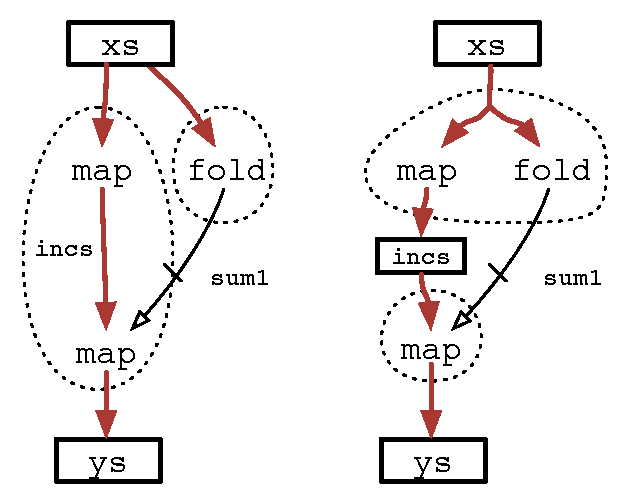
\includegraphics[scale=0.5]{figures/ex2-normalizeInc.pdf}
\end{center}
\caption{Possible clusterings for \texttt{normalizeInc}}
\label{f:normalizeInc}
\end{figure}


% -----------------------------------------------------------------------------
\section{Integer Linear Programming}
\label{s:ILP}
It is usually possible to cluster a program graph in multiple ways. For example, consider the following simple function:
\begin{code}
 normalizeInc :: Array Int -> Array Int
 normalizeInc xs
  = let incs = map  (+1)     us
        sum1 = fold (+) 0    us
        ys   = map  (/ sum1) incs
    in  ys
\end{code}

Two possible clusterings are shown in Figure~\ref{f:normalizeInc}. One option is to compute @sum1@ first and fuse the computation of @incs@ and @ys@. Another option is to fuse the computation of @incs@ and @sum1@ into a single loop, then compute @ys@ separately. A third option (not shown) is to compute all results separately, and not perform any fusion. 

Which option is better? On current hardware we generally expect the cost of memory access to dominate runtime. The first clustering in Figure~\ref{f:normalizeInc} requires two reads from array @xs@ and one write to array @ys@. The second requires a single fused read from @xs@, one write to @incs@, a read back from @incs@ and a final write to @ys@. From the size constraints of the program we know that all intermediate arrays have the same size, so we expect the first clustering will peform better as it only needs three array accesses instead of four. 

For small programs such as @normalizeInc@ it is possible to naively enumerate all possible clusterings, select just those that are \emph{valid} with respect to fusion preventing edges, and choose the one that maximises a cost metric such as the number of array accesses needed. However, as the program size increases the number of possible clusterings becomes too large to naively enumerate. For example, Pouchet et al~\cite{pouchet2010combined} present a fusion system using the polyhedral model~\cite{pouchet2011polyhedral} and report that some simple numeric programs have over 40,000 possible clusterings, with one particular example having $10^{12}$. 

To deal with the combinatorial explosion in the number of potential clusterings, we instead use an Integer Linear Programming (ILP) formulation. ILP problems are defined as a set of variables, an objective linear function and a set of linear constraints. The integer linear solver finds an assignment to the variables that minimises the objective function, while satisfying all constraints. For the clustering problem we express our constraints regarding fusion preventing edges as linear constraints on the ILP variables, then use the objective function to encode our cost metric. This general approach was first fully described by Megiddo and Sarkar~\cite{megiddo1998optimal}, and our main contribution is to extend it to work with size changing operators such as @filter@. 


% -----------------------------------------------------------------------------
\subsection{Dependency Graphs}
A dependency graph represents the data dependencies of the program to be fused, and we use it as an intermediate stage when producing linear constraints for the ILP problem. The dependency graph contains enough information to determine the possible clusterings of the input program, while abstracting away from the exact operators used to compute each intermediate array. The rules for producing dependency graphs are in Figure~\ref{f:DependencyGraph}.

Each binding in the source program becomes a node in the dependency graph. For each intermediate variable, we add a directed edge from the binding that produces a value to all bindings that consume it. Each edge is also marked as either \emph{fusible} or \emph{fusion preventing}. Fusion preventing edges are used when the producer must finish its execution before the consumer node can start. For example, a @fold@ operation must complete execution before it can produce the scalar value needed by its consumers. Conversely, the @map@ operation produces an output value for each value it consumes, so is marked as fusible. 

The @gather@ operation is a hybrid: it takes an indices array and an elements array, and for each element in the indices array returns the corresponding data element. This means that gather can be fused with the operation that produces its indices, but not the operation that produces its elements --- because those are accessed in a random-access manner. 

\begin{figure}
\begin{tabbing}
MMMMM       \= M  \= \kill
$nodes$     \> @:@ \> $\program \to V$                          \\
$edges$     \> @:@ \> $\program \to E$                          \\
$edge$      \> @:@ \> $\{bind\} \times bind \to E$              \\
$inedge$    \> @:@ \> $\{bind\} \times name \times name \to E$
\\[1ex]
$nodes(bs)$ \> $= \{(name(b), \iiter_{\Gamma,C}(b)) | b \in bs\}$
\\[1ex]
$edges(bs)$ \> $= \bigcup_{b \in bs}edge(bs, b)$
\\[1ex]
MM             \= M \= \kill
$edge(bs, out = @fold@~f~in)$ \\
    \> $=$    \> $\{inedge(bs,out,s) | s \in fv(f)\} \cup \{inedge(bs, out, in) \}$
\\
$edge(bs, out = @map@~f~in)$  \\
    \> $=$    \> $\{inedge(bs,out,s) | s \in fv(f)\} \cup \{inedge(bs, out, in) \}$
\\
$edge(bs, out = @filter@~f~in)$ \\
    \> $=$    \> $\{inedge(bs,out,s) | s \in fv(f)\} \cup \{inedge(bs, out, in) \}$
\\
$edge(bs, out = @gather@~data~indices)$ \\
    \> $=$    \> $\{(out,data, \fusionpreventing) \} \cup \{inedge(bs, out, indices) \}$      
\\
$edge(bs, out = @cross@~a~b)$ \\
    \> $=$    \> $\{inedge(bs, out, a) \}           \cup      \{(out, b, \fusionpreventing) \}$
\\
$edge(bs, outs = @external@~ins)$  \\
    \> $=$    \> $\{(outs,i, \fusionpreventing) | i \in ins \}$
\\[1ex]
$inedge(bs,to,\from)$ \\
    \> $|$ \> $(\from = @fold@~f~s) \in bs$     \\
    \> $=$ \> $(to, \from, \fusionpreventing)$  \\
    \> $|$ \> $(outs = @external@ \ldots) \in bs     \wedge \from \in outs$     \\
    \> $=$ \> $(to, outs, \fusionpreventing)$  \\
    \> $|$ \> $otherwise$                      \\
    \> $=$ \> $(to, \from, \fusible)$
\end{tabbing}

\caption{Dependency Graphs from Programs}
\label{f:DependencyGraph}
\end{figure}


% -----------------------------------------------------------------------------
\subsection{ILP Variables}
After generating the dependency graph, the next step is to produce a set of linear constraints from this graph. The variables involved in these constraints are split into three groups:
\begin{tabbing}
M   \= MM \= MMMMMMM \= MM \= \kill
$x$   \> @:@  \> $node \times node$ \> $\to$ \> $\mathbb{B}$
\end{tabbing}

For each pair of nodes with indices $i$ and $j$ we use a boolean variable $x_{i,j}$ which indicates whether those two nodes are fused. We use $x_{i,j} = 0$ when the nodes are fused and $x_{i,j} = 1$ when they are not. Using $0$ for the fused case means that the objective function can be a weighted function of the $x_{i,j}$ variables, and minimizing it tends to increase the number of nodes that are fused. The values of these variables are used to construct the final clustering, such that $\forall i,j.\ x_{i,j} = 0 \iff cluster(i) = cluster(j)$.
\begin{tabbing}
M   \= MM \= MMMMMMM \= MM \= \kill
$\pi$ \> @:@  \> $node$             \> $\to$ \> $\mathbb{R}$
\end{tabbing}

The second group of variables is used to ensure that the clustering is acyclic. This means that for each node in the graph, the dependencies of that node can be executed before the node itself. For each node $i$, we associate a real $\pi_i$ such that every node $j$ that depends on $i$ we have $\pi_j > \pi_i$. Our linear constraints will ensure that if two nodes are fused into the same cluster then their $\pi$ values will be identical --- though nodes in different clusters can also have the same $\pi$ value. Here is an example of a cyclic clustering:
\begin{code}
  cycle xs  = let ys  = map (+1) xs     (C1)
                  sum = fold ys         (C2)
                  zs  = map (+sum) ys   (C1)
              in  zs
\end{code}

There is no fusion-preventing edge directly between the @xs@ and @zs@ bindings, but there is a fusion-preventing edge between @sum@ and @zs@. If the @xs@ and @zs@ bindings were in the same cluster @C1@ and @sum@ was in cluster @C2@, there would be a dependency cycle between @C1@ and @C2@, and neither could be executed before the other.
\begin{tabbing}
M   \= MM \= MMMMMMM \= MM \= \kill
$c$   \> @:@  \> $node$             \> $\to$ \> $\mathbb{B}$
\end{tabbing}

The final group of variables is used to help define the cost model encoded by the objective function. Each node is assigned a variable $c_i$ that indicates whether the array the associated binding produces is \emph{fully contracted}. When an array is fully contracted it means that all consumers of that array are fused into the same cluster, so we have $c_i = 0 \iff \forall (i',j) \in E.\ i = i' \implies x_{i,j} = 0$. In the final program, each successive element of a fully contracted array can be stored in a scalar register, rather than requiring an array register or memory storage. 


% -----------------------------------------------------------------------------
\subsection{Linear Constraints}
\label{s:LinearConstraints}
The constraints we place on the ILP variables are split into four groups: constraints that ensure the clustering is acyclic; constraints that encode fusion preventing edges; constraints on nodes with different iteration sizes, and constraints involving array contraction. 

% -------------------------------------
\paragraph{Acyclic and precedence-preserving} The first group of constraints ensures that the clustering is acyclic:
\begin{tabbing}
MM  \= MMMx \= M \= MMM \= M \= MMMM \= \kill
    \> ~~~~~~~ $x_{i,j}$ \> $\le$ \> $\pi_j - \pi_i$ \> $\le$ \> $N \cdot x_{i,j}$ 
    \>             (with an edge from $i$ to $j$)            \\
    \> $-N \cdot  x_{i,j}$  \> $\le$ \> $\pi_j - \pi_i$ \> $\le$ \> $N \cdot x_{i,j}$ 
    \>             (with no edge from $i$ to $j$)
\end{tabbing}

As per Megiddo~\cite{megiddo1998optimal} the form of these constraints is determined by whether there is an dependency between nodes $i$ and $j$. The $N$ value is set to the total number of nodes in the graph.

If there is an edge from node $i$ to $j$ we use the first constraint form shown above. If the two nodes are fused into the same cluster then we have $x_{i,j} = 0$. In this case the constraint simplifies to $0 \le \pi_j - \pi_i \le 0$, which forces $\pi_i = \pi_j$. If the two nodes are in \emph{different} clusters then the constraint instead simplifies to $1 \le \pi_j - \pi_i \le N$. This means that the difference between the two $\pi$s must be at least 1, and less than $N$. Since there are $N$ nodes, the maximum difference between any two $\pi$s would be at most $N$, so the upper bound of $N$ is large enough to be safely ignored. This means the constraint can roughly be translated to $\pi_i < \pi_j$, which enforces the acyclicity constraint.

If instead there is no edge from node $i$ to $j$ then we use the second constraint form above. As before, if the two nodes are fused into the same cluster then we have $x_{i,j} = 0$, which forces $\pi_i = \pi_j$. If the nodes are in different clusters then the constraint simplifies to $-N \le \pi_j - \pi_i \le N$, which effectively puts no constraint on the $\pi$ values.


% -------------------------------------
\paragraph{Fusion-preventing edges} As per Megiddo~\cite{megiddo1998optimal}, if there is a fusion preventing edge between two nodes we add a constraint to ensure the nodes will be placed in different clusters.
\begin{tabbing}
MMM     \= MMM \= M  \= MMM \= M \= MMM \= \kill
        \> $x_{i,j}$ \> $=$ \> $1$ \>   \> \\
        \> (for fusion-preventing edges from $i$ to $j$) 
\end{tabbing}

When combined with the precedence-preserving constraints earlier, setting $x_{i,j} = 1$ also forces $\pi_i < \pi_j$. 


% -------------------------------------
\paragraph{Fusion between different iteration sizes} This group of constraints restricts which nodes can be placed in the same cluster based on their iteration size. The group has three parts. 
Firstly, either of the two nodes connected by an edge have an unknown ($\bot$) iteration size then they cannot be fused and we set $x_{i,j} = 1$:
\begin{tabbing}
MMM     \= MMM \= M \= MMM \= M \= MMM \= \kill
        \> $x_{i,j}$   \> $=$   \> $1$          \>       \>     \\
        \> (if $\iiter_{\Gamma,C}(i) = \bot 
                ~\vee~ \iiter_{\Gamma,C}(j) = \bot$)
\end{tabbing}

Secondly, if the two nodes have different iteration sizes and no common parent then they also cannot be fused and we set $x_{i,j} = 1$:
\begin{tabbing}
MMM     \= MMM \= M \= MMM \= M \= MMM \= \kill
        \> $x_{i,j}$   \> $=$   \> $1$          \>       \>     \\
        \> (if $\iiter_{\Gamma,C}(i) \not= \iiter_{\Gamma,C}(j) 
                ~\wedge~ parents(i,j) = \emptyset$)
\end{tabbing}

Finally, if the two nodes had different iteration sizes but \emph{do} have parent transducers of the same size, then the two nodes can be fused if they are fused with their respective parents, and the parents themselves are fused:
\begin{tabbing}
MMM     \= MMM \= M \= MMM \= M \= MMM \= \kill
        \> $x_{a,A}$   \> $\le$ \> $x_{a,b}$    \>       \>     \\
        \> $x_{b,B}$   \> $\le$ \> $x_{a,b}$    \>       \>     \\
        \> $x_{A,B}$   \> $\le$ \> $x_{a,b}$    \>       \>     \\
        \> (if $\iiter_{\Gamma,C}(a) \not= \iiter_{\Gamma,C}(b) 
                ~\wedge~ parents(a,b) = \{(A,B)\}$)
\end{tabbing}

This last part is the main difference to existing ILP solutions: we allow nodes with different iteration sizes to be fused when their parent transducers are fused. The actual constraints encode a ``no more fused than'' relationship. For example $x_{a,A} \le x_{a,b}$ means that nodes $a$ and $b$ can be no more fused than nodes $a$ and $A$. 

As a simple example, consider fusing an operation on filtered data with its generating filter:
\begin{code}
    sum1 = fold (+) 0  xs
    gts  = filter (>0) xs
    sum2 = fold (+) 0  gts
\end{code}

Here $sum1$ and $sum2$ have different iteration sizes and we have that $parents(sum1, sum2) = \{(sum1, gts)\}$. This means that $sum1$ and $sum2$ may only be fused if $sum1$ is fused with $sum1$ (trivial), $sum2$ is fused with $gts$, and $sum1$ is fused with $gts$.


% -------------------------------------
\paragraph{Array contraction} The final group gives meaning to the $c$ variables, which represent whether an array is fully contracted:
\begin{tabbing}
MMM     \= MMM \= M \= MMM \= M \= MMM \= \kill
        \> $x_{i,j}$    \> $\le$ \> $c_i$  \> \> \\
        \> (for all edges from i)
\end{tabbing}

Recall that an array is fully contracted when all of the consumers are fused with the nodes that produces it, which means that the array does not need to be fully materialized in memory. As per Darte's work on array contraction~\cite{darte2002contraction}, we define a variable $c_i$ for each array, and the constraint above ensures that $c_i = 0$ only if $\forall (i',j) \in E.\ i = i' \implies x_{i,j} = 0$. By minimizing $c_i$ in the objective function, we favor solutions that reduce the number of intermediate arrays.


% -----------------------------------------------------------------------------
\subsection{Objective Function}
\label{s:ObjectiveFunction}
The objective function defines the cost model of the program, and the ILP solver will find the clustering that minimizes this function while satisfying the constraints defined in the previous section. The cost model we use in this paper has three components:
\begin{itemize}
\item
the number of array reads and writes --- an abstraction of the amount of memory bandwidth needed by the program; 
\item
the number of intermediate arrays --- an abstraction of the amount of intermediate memory needed; 
\item
the number of distinct clusters --- an abstraction of the cost of loop management instructions, which maintain loop counters and the like.
\end{itemize}

The three components of the cost model are a heuristic abstraction of the true cost of executing the program on current hardware. They are ranked in order of importance --- so we prefer to minimize the number of array reads and writes over the number of intermediate arrays, and to minimize the number of intermediate arrays over the number of clusters. However, minimizing one component does not necessarily minimize any other. For example, as the fused program executes multiple array operations at the same time, in some cases the clustering that requires the least number of array reads and writes uses more intermediate arrays than strictly necessary.

We encode the ordering of the components of the cost model as different weights in the objective function. First, note that if the program graph contains $N$ combinators (nodes) then there are at most $N$ opportunities for fusion. We then encode the relative cost of loop overhead as weight $1$, the cost of an intermediate array as weight $N$, and the cost of an array read or write as weight $N^2$. This ensures that no amount of loop overhead reduction can outweigh the benefit of removing an intermediate array, and likewise no number of removed intermediate arrays can outweigh a reduction in the number of array reads or writes. The integer linear program including the objective function is as follows:
\begin{tabbing}
MMMMM   \= MMMM \= M \= \kill
Minimise   \>     $\Sigma_{(i,j) \in E} W_{i,j} \cdot x_{i,j}$   
                        ~~ (memory traffic and loop overhead)
\\ ~~~~~~~~~~~~~ $+$ \> $\Sigma_{i \in V} N \cdot c_i$
                        ~~~~~~~~~~~~ (removing intermediate arrays)
\\[1ex]
   Subject to  \> \ldots ~ constraints from \S\ref{s:LinearConstraints} ~ \ldots 
\\ Where   \> $W_{i,j} = N^2$ \> $~|$ \> $(i,j) \in E $         
\\         \> \> \> (fusing $i$ and $j$ will reduce memory traffic)         
\\         \> $W_{i,j} = N^2$ \> $~|$ \> $\exists k. (k,i) \in E \wedge (k,j) \in E $     
\\         \> \> \> ($i$ and $j$ share an input array)
\\         \> $W_{i,j} = 1$   \> $~|$ \> $@otherwise@$
\\         \> \> \> (the only benefit is loop overhead)
\\         \> $N = |V|$
\end{tabbing}


% -----------------------------------------------------------------------------
\subsection{Fusion-preventing Path Optimisation}
\label{s:OptimisedConstraints}
The integer linear program defined in the previous section includes more constraints than strictly necessary to define the valid clusterings. If two nodes have a path between them which includes a fusion preventing edge, then we know up front that they must be placed in different clusters. The following function $possible(a,b)$ determines whether there is any possibility that the two nodes $a$ and $b$ can be fused. Similarly the function $possible'(a, b)$ checks whether there is any possibility that the parents of $a$ and $b$ may be fused.
%
\begin{tabbing}
MMMM \= M \=     \= MMMMMMMMMMMM    \=  \kill
$possible$ \> $:$     \> $name \times name \to \mathbb{B}$      \\
MMMMMMx        \= M    \= \kill
$possible(a,b)$   
        \> $=$  \>$\forall p \in path(a,b) \cup path(b,a).\ \fusionpreventing \not\in p$
\\[1ex]
MMMM \= M \=     \= MMMMMMMMMMMM    \=  \kill
$possible'$     \> $:$ \> $name \times name \to \mathbb{B}$      \\
MMMMMMx        \= M    \= \kill
$possible'(a,b)$ 
        \> $=$   \>$\exists A, B.\  parents(a,b) = \{A,B\} \wedge possible(a,b)$ \\
        \> $\wedge$ \> $possible(A,a) \wedge possible(B,b) \wedge possible(A,B)$
\end{tabbing}

With $possible$ and $possible'$ defined, we refine our formulation to only generate constraints between two nodes if there is a chance they may be fused together. Doing this reduces the total number of constraints, and makes the job of the ILP solver easier. The final formulation of the integer linear program follows.
%
\begin{tabbing}
MMMMM   \= MMMM \= M \= MMMM \= M \= MMMM \= \kill
Minimise   \> $\Sigma_{(i,j) \in E} W_{i,j} \cdot x_{i,j} + \Sigma_{i \in V} N \cdot c_i$  \\
           \> (if $possible(i,j)$)         
\\[0.5ex]
Subject to \> $-N \cdot x_{i,j}$ \> $\le$ \> $\pi_j - \pi_i$ \> $\le$ \> $N \cdot x_{i,j}$ \\
           \> (if $possible(i,j) \wedge (i,j) \not\in E \wedge (j,i) \not\in E$)            
\\[0.5ex]
           \>    $x_{i,j}$ \> $\le$ \> $\pi_j - \pi_i$ \> $\le$ \> $N \cdot x_{i,j}$ \\
           \> (if $possible(i,j) \wedge (i,j,\fusible) \in E$)     
\\[0.5ex]
           \>             \>       \> $\pi_i < \pi_j$ \>       \>            \\
           \> (if $(i,j,\fusionpreventing) \in E$)    
\\[0.5ex]
           \> $x_{i,j}$    \> $\le$ \> $c_i$           \>       \>            \\
           \> (if $(i,j, \fusible) \in E$) \\
           \> $c_{i }$    \> $ = $ \> $ 1 $           \>       \>            \\
           \> (if $(i,j, \fusionpreventing) \in E$)
\\[0.5ex]
           \> $x_{i,j}$    \> $=$   \> $1$             \>       \>            \\
           \> (if $\bot \in \{\iiter_{\Gamma,C}(i), \iiter_{\Gamma,C}(j)\}$)  
\\[0.5ex]
           \> $x_{i',i}$   \> $\le$ \> $x_{i,j}$        \>       \>            \\
           \> $x_{j',j}$   \> $\le$ \> $x_{i,j}$        \>       \>            \\
           \> $x_{i',j'}$   \> $\le$ \> $x_{i,j}$        \>       \>            \\
           \> (if $\iiter_{\Gamma,C}(i) \not= \iiter_{\Gamma,C}(j) \wedge possible'(i,j)$ \\
           \> \> $\wedge~parents(i,j) = \{(i',j')\}$) 
\\[0.5ex]
           \> $x_{i,j}$    \> $=$   \> $1$             \>       \>            \\
           \> (if $\iiter_{\Gamma,C}(i) \not= \iiter_{\Gamma,C}(j) \wedge \neg possible'(i,j)$) 
\\[0.5ex]
MMMMM   \= MMMM \= M \= \kill
Where      \> $W_{ij} = N^2$ \> $~|$ \> $(i,j) \in E $         \\
           \> \> \> (fusing $i$ and $j$ will reduce memory traffic)         \\
           \> $W_{ij} = N^2$ \> $~|$ \> $\exists k. (k,i) \in E \wedge (k,j) \in E $     \\
           \> \> \> ($i$ and $j$ share an input array)                                         \\
           \> $W_{ij} = 1$   \> $~|$ \> $@otherwise@$                                                  \\
           \> \> \> (the only benefit is loop overhead)                                        
\\
           \> $N = |V|$
\end{tabbing}

% % !!!!!!!!!!!!!!!!!!!!!!!
% I commented the \input out in section/04-ILP.tex

\subsection{Proof}
To prove correctness of our linear program formulation, we need to prove two different things.
Firstly, the formulation's constraints must always be satisfiable; that is, there must exist a variable assignment that satisfies all constraints.
This is rather simple to show, but guarantees that the linear program will always give an answer.
The next thing to show is that any produced clustering is legal: if a variable assignment satisfies the constraints, then it is a valid and legal clustering.
This means that, not only do we get \emph{an} answer, we also get the \emph{right} answer.

%!TEX root = ../Main.tex
\subsubsection{Satisfiability}
For any program $p$, there exists a trivial clustering with no fusion at all.
We can use this as the variable assignment of $ilp(p)$.
For each pair of nodes $m,n \in p$, $x_{mn} = 1$ --- no fusion is possible.
For the $\pi$ variables, we must find a topographical ordering of the nodes in $p$, which is simple since we are assured it is a dag.

\TODO{Now, prove that this assignment actually satisfies the constraints.}


\subsubsection{Soundness}
For any program $p$ and variable asignment $v$, if $v$ satisfies the constraints for $ilp(p)$, the clustering denoted by $x_{ij}$ in $v$ is legal.

For a clustering to be legal, it must satisfy three constraints:
\begin{description}
\item[Acyclic]
after merging nodes of same cluster together, the resulting graph must be a dag
\item[Precedence preserving]
if there is an edge between two nodes $i$ and $j$, and they are not merged together, then we require $\pi_j > \pi_i$
\item[Fusion preventing]
likewise, if there is a fusion-preventing edge between two nodes $i$ and $j$, then we require $\pi_j > \pi_i$, which implies that they are not merged together
\item[Type constraint]
if two nodes $i$ and $j$ are in the same cluster, then $\tau_i = \tau_j$, or if $\tau_i$ is a subtype of $\tau_j$ (or $\tau_j$ is a subtype of $\tau_i$), then the \emph{generator} for $\tau_i$ (or $\tau_j$) must also be in the same cluster as $i$ and $j$.
    \\
    \TODO Actually, let us say $x_{ij} = 0 \implies check_{ij}$

\end{description}
where
\begin{tabbing}
MMMMM      \= M \= MMMMMMM \= MM \= \kill
$check$ \> @::@  \> $array \times array$ \> $\to$ \> $\mathbb{B}$ \\
MMMMM      \= M \= MMMMMM \= MM \= \kill
$check(i, j)$     \> $|$ \> $tau_i = tau_j$ \> $=$ \> $x_{i,j} = 0$                        \\
$check(i, j)$     \> $|$ \> $i' \in gen(i) $ \> $=$ \> $x_{i',j} = 0 \wedge x_{i,i'} = 0 \wedge check(i', j)$                        \\
$check(i, j)$     \> $|$ \> $j' \in gen(j) $ \> $=$ \> $x_{i,j'} = 0 \wedge x_{j,j'} = 0 \wedge check(i, j')$                        \\
$check(i, j)$     \> $|$ \> $tau_i \not= tau_j$\> $=$ \> $\bot$
\end{tabbing}









%!TEX root = ../Main.tex
\clearpage{}
\section{Benchmarks}

\begin{figure}
\begin{code}

\end{code}
\caption{Analytic Operators}
\end{figure}

%!TEX root = ../acc-optim.tex
\section{Related work} % (fold)
\label{sec:related}
Repa \cite{Keller:Repa} is a Haskell library for parallel array programming on shared-memory SMP machines. Repa uses the \mbox{delayed/manifest} representation split on which our @DelayedAcc@ type is based, though the idea of representing arrays as functions is folklore. With Repa the conversion between array representations is done manually and can cause shared expressions to be recomputed rather than stored. Such recomputation can improve runtime performance depending on the algorithm. In Accelerate the conversion is automatic and conservative, so that shared expressions are never recomputed. 

Vertigo~\cite{Elliott:Vertigo}, Nikola \cite{Mainland:nikola} and Obsidian \cite{Claessen:obsidian} are EDSLs in Haskell and were mentioned in Section~\ref{sec:Introduction}. Vertigo is a first-order language for writing shaders, and does not provide higher-order combinators such as @map@ and @fold@. Nikola uses an instance of Gill's approach~\cite{Gill:2009dx} to sharing recovery, is limited to single GPU kernel programs, and performs no fusion. 

Obsidian~\cite{Claessen:obsidian} is a lower level language where more details of the GPU hardware are exposed to the programmer. Recent versions of Obsidian \cite{Claessen:obsidian-expressive} implement Repa-style delayed \emph{pull arrays} as well as \emph{push arrays}. Whereas a pull array represents a general producer, a push array represents a general consumer. Push arrays allow the intermediate program to be written in continuation passing style (CPS), and helps to compile (and fuse) append-like operations.

Baracuda~\cite{Larsen:baracuda} is another Haskell EDSL that produces CUDA GPU kernels, though is intended to be used offline, with the kernels being called directly from C++. The paper~\cite{Larsen:baracuda} mentions a fusion system that appears to be based on pull arrays, though the mechanism is not discussed in detail. Barracuda steps around the sharing problem by requiring let-bindings to be written using the AST node constructor, rather than using Haskell's native let-expressions.

Delite/LMS~\cite{Rompf-etal:Delite} is a parallelisation framework for DSLs in Scala that uses library-based multi-pass staging to specify complex optimisations in a modular manner. Delite supports loop fusion for DSLs targeting GPUs using rewrite rules on a graph-based IR.

NDP2GPU~\cite{bergstrom:ndp2gpu} compiles NESL code down to CUDA. As the source language is not embedded there is no need for sharing recovery. NDP2GPU performs @map@/@map@ fusion but cannot fuse @map@s into reduction combinators.

Sato and Iwasaki~\cite{Sato:Skeletal-fusion} describe a C++ library for GPGPU programming that includes a fusion mechanism based on list homomorphisms~\cite{Meijer:bananas}. The fusion transformation itself is implemented as a source to source translation. SkeTo \cite{Matsuzaki:Skeletal-expression-templates} is a C++ library that provides parallel skeletons for CPUs. SkeTo's use of C++ templates provides a fusion system similar to delayed arrays, which could be equivalently implemented using CUDA templates. The authors of SkeTo note that the lack of type inference in C++ leads them to write their array code as nested expressions --- to avoid intermediate variable bindings and their required type annotations.

% section related (end)



\section*{Acknowledgements}
Many thanks are due to
Manuel Chakravarty,
Robert Clifton-Everest,
Erik de Castro Lopo,
Kai Engelhardt,
Bill Kroon,
Frederik M.\ Madsen,
Abdallah Saffidine,
Carter Schonwald,
and Jingling Xue
for enlightening discussions relating to this work.

\bibliographystyle{plain}
\bibliography{Main}

\end{document}


